% !TeX root = ../../../main.tex
\subsection{Additional Informative Censoring via Unobserved Confounding}
\label{ch04:app:informative-censoring-uconf}
In the main paper, we model informative censoring by making censoring times stochastically dependent on event times, reflecting realistic scenarios where patients with shorter expected survival may drop out earlier. 
Here we complement this setting with an alternative mechanism where the ignorable censoring assumption is violated due to unobserved confounding. 
This extension demonstrates the flexibility of our modular data generation framework.

\ChFourParagraph{Data generation process.}
We follow the same covariate generation procedure as in our synthetic datasets: observed covariates $X \sim \text{Uniform}(0,1)^5$ and an unobserved covariate $U \sim \text{Uniform}(0,1)$. 
Treatment assignment follows the \texttt{OBS-UConf} configuration, where $U$ enters into both treatment assignment and outcome generation but remains unobserved during estimation. 

We focus on survival Scenario~\texttt{C} (Poisson hazards with medium censoring).
Event times and censoring times are generated as follows, where $w \in \{0,1\}$ is the treatment indicator:
\begin{align}
    \lambda(w) &= X_2^2 + X_3 + 6 + 2\left(\sqrt{0.3 \cdot X_1 + 0.7 \cdot U} - 0.3\right) \cdot w + \epsilon, \\
    T(w) &\sim \text{Poisson}(\lambda(w)), \\
    C &= 
    \begin{cases} 
      \infty & \text{if } U \leq 0.6, \\[0.5em]
      1 + \ChFourInd(X_{4} < 0.5) & \text{otherwise},
    \end{cases}
\end{align}
where $\epsilon \sim \mathcal{N}(0,0.1)$ adds stochastic variation. 
The censoring distribution thus depends directly on the unobserved variable $U$, creating dependence between censoring and survival that cannot be explained away by the observed $X$ alone. 

\ChFourParagraph{Summary statistics}
Similar to the other synthetic datasets, we include up to 50{,}000 samples with treatment assigned according to an observational study mechanism. 
The treatment rate is 53.9\%, the censoring rate is 39.7\% (driven by $U$), and the population-level ATE is 0.7737 (computed from the 50,000 samples by averaging the CATEs). 
This setup mirrors real-world contexts such as clinical trials with dropout patterns influenced by latent health status.

\ChFourParagraph{Experimental results}
We evaluated representative estimators from all three method families. 
Figure~\ref{ch04:fig:uconf-ic-results} reports CATE RMSE and ATE bias (mean $\pm$ standard error) across 10 random splits. 




% !TeX root = ../../../main.tex
\begin{figure}[htbp]
\ChFourFloatContents{ch04:fig:uconf-ic-results}{\caption{CATE RMSE (left) and ATE bias (right) under informative censoring induced by unobserved confounding.}}{
    \centering

\resizebox{1\textwidth}{!}{%
        \begin{minipage}{1\textwidth}

    \subfloat[{RCT:\ChFourBlackCross, Ignorability:\ChFourBlackCross, Positivity:\ChFourGrayCheck, Ignorable Censoring:\ChFourBlackCross}]{\begin{minipage}[t]{0.49\textwidth}
        \centering
        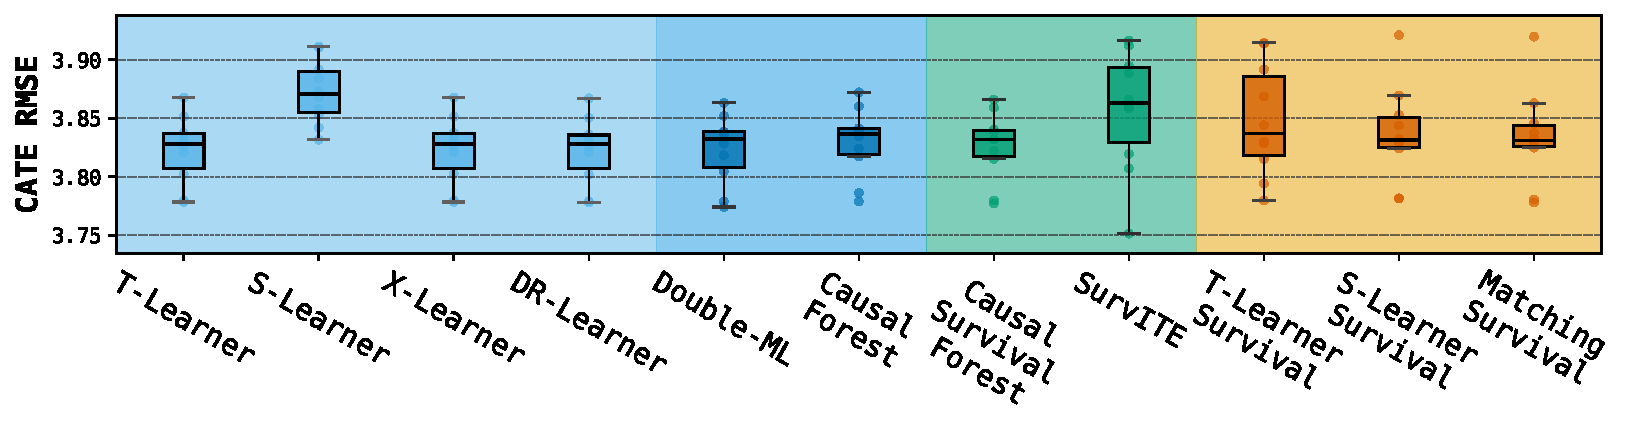
\includegraphics[width=\linewidth]{Appendices/appendix-ch04/images/figure_results_updated/unobIC_scenario_C_e_X_U_info_censor_unobserved_cate_rmse.pdf} 
       
    \end{minipage}}
    \hfill
    \subfloat[{RCT:\ChFourBlackCross, Ignorability:\ChFourBlackCross, Positivity:\ChFourGrayCheck, Ignorable Censoring:\ChFourBlackCross}]{\begin{minipage}[t]{0.49\textwidth}
        \centering
        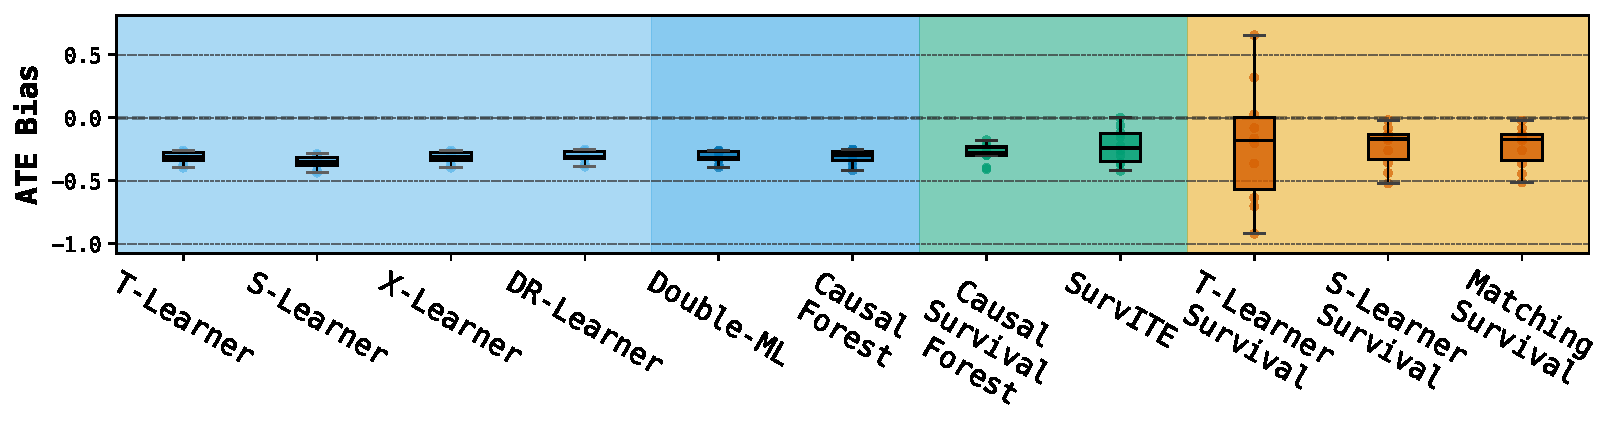
\includegraphics[width=\linewidth]{Appendices/appendix-ch04/images/figure_results_updated/unobIC_scenario_C_e_X_U_info_censor_unobserved_ate_bias.pdf} 
        
    \end{minipage}}
    \end{minipage}%
    }
    
    
    
}
\end{figure}


The results indicate that Causal Survival Forests and survival meta-learners with matching tend to perform best under this setting, consistent with findings from the main synthetic datasets. 

\ChFourParagraph{Extensibility to other settings.}
Here we illustrate one case: \texttt{OBS-UConf} combined with Scenario~\texttt{C}.  
However, the same mechanism can be straightforwardly extended to other causal configurations (e.g., randomized trials with imbalance) and survival scenarios (e.g., AFT or Cox models).  
We leave systematic exploration of these additional combinations for future work, but their ease of inclusion highlights the flexibility of \textsc{SurvHTE-Bench} to accommodate alternative censoring mechanisms.%




